\begin{DensePanel}{300mm}{6}{THE USUAL COMPENSATION MAKES IT WORSE}
  \begin{center}
    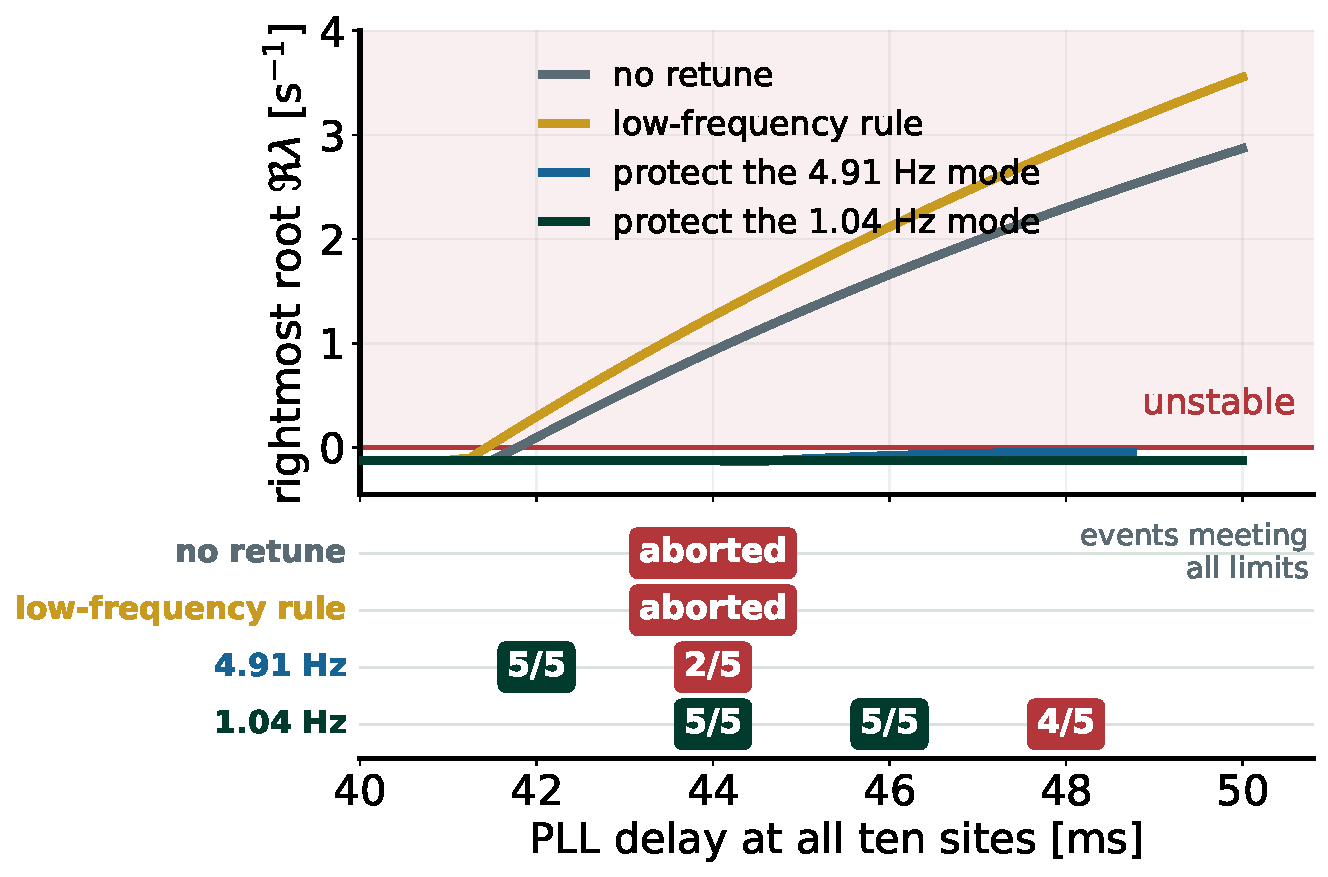
\includegraphics[width=272mm,height=196mm,keepaspectratio]{generated/figures/central.pdf}
  \end{center}
  \vspace{-1mm}
  \noindent{\DenseBig\color{IASVermillion}12 vs 0}\hspace{4mm}%
  \begin{minipage}[b]{168mm}{\DenseSmall\raggedright unstable roots at 44 ms: the low-frequency rule against protecting the 1.04 Hz mode (full-spectrum count).\par}\end{minipage}\par
  \vspace{2mm}
  \begin{DenseWords}\textbf{\color{IASGold!65!black}IN WORDS\ \ }Which mode you protect decides everything. Protecting the 4.91 Hz mode keeps the spectrum but fails 3 of 5 events; protecting the 1.04 Hz mode passes 5 of 5.\end{DenseWords}
\end{DensePanel}
